\definecolor{cases-default}{HTML}{EB5353}
\definecolor{controls-default}{HTML}{0079FF}
\definecolor{healthy-default}{HTML}{36AE7C}
\definecolor{baseline}{HTML}{FAEAB1}
\definecolor{preds}{HTML}{E5BA73}
\definecolor{maps}{HTML}{C58940}

\def\marksize{8pt}

\newsavebox{\resultsbox}
    \sbox{\resultsbox}{%
    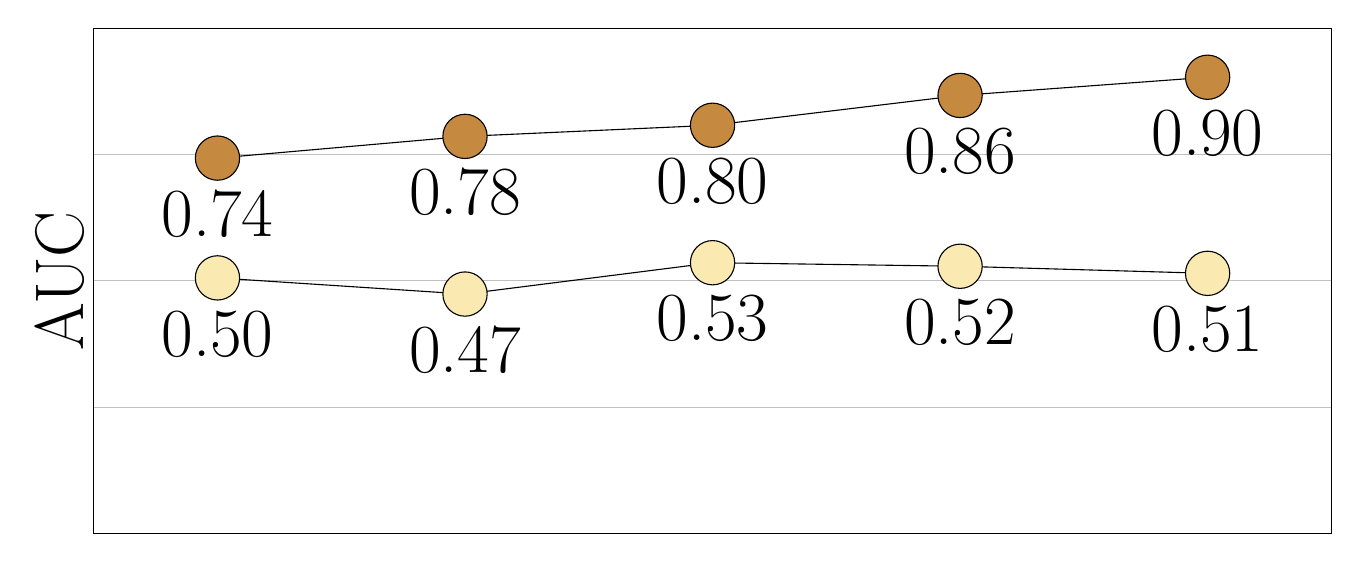
\begin{tikzpicture}
        \begin{axis}[
            height=8cm,
            width=17.3cm,
            xmajorticks=false,
            xmin=0.5,
            xmax=5.5,
            ymin=0,
            ymax=1,
            ylabel=AUC,
            ymajorticks=false,
            ymajorgrids=true,
            ytick={0.25, 0.50, 0.75},
            axis background/.style={fill=white},
            label style={font=\fontsize{32}{32}\selectfont}
        ]
            \addplot[mark=*, draw=black, mark options={fill=baseline}, mark size=\marksize] coordinates {
                (1, 0.506)
                (2, 0.474)
                (3, 0.536)
                (4, 0.529)
                (5, 0.515)
            };\label{trace:baseline}
            \addplot[mark=*, draw=black, mark options={fill=maps}, mark size=\marksize] coordinates {
                (1, 0.743)
                (2, 0.786)
                (3, 0.808)
                (4, 0.867)
                (5, 0.903)
            };\label{trace:maps}
            \node[anchor=north, inner sep=12pt, font=\fontsize{24}{24}\selectfont] at (axis cs: 1, 0.506) {0.50};
            \node[anchor=north, inner sep=12pt, font=\fontsize{24}{24}\selectfont] at (axis cs: 2, 0.474) {0.47};
            \node[anchor=north, inner sep=12pt, font=\fontsize{24}{24}\selectfont] at (axis cs: 3, 0.536) {0.53};
            \node[anchor=north, inner sep=12pt, font=\fontsize{24}{24}\selectfont] at (axis cs: 4, 0.529) {0.52};
            \node[anchor=north, inner sep=12pt, font=\fontsize{24}{24}\selectfont] at (axis cs: 5, 0.515) {0.51};
            \node[anchor=north, inner sep=12pt, font=\fontsize{24}{24}\selectfont] at (axis cs: 1, 0.743) {0.74};
            \node[anchor=north, inner sep=12pt, font=\fontsize{24}{24}\selectfont] at (axis cs: 2, 0.786) {0.78};
            \node[anchor=north, inner sep=12pt, font=\fontsize{24}{24}\selectfont] at (axis cs: 3, 0.808) {0.80};
            \node[anchor=north, inner sep=12pt, font=\fontsize{24}{24}\selectfont] at (axis cs: 4, 0.867) {0.86};
            \node[anchor=north, inner sep=12pt, font=\fontsize{24}{24}\selectfont] at (axis cs: 5, 0.903) {0.90};
        \end{axis}
    \end{tikzpicture}
}
\begin{figure}
    \begin{tikzpicture}
        \begin{axis}[
            height=0.45\textwidth,
            width=0.9\textwidth,
            xlabel=Age,
            ylabel=Cognitive function,
            ticks=none,
            axis x line=bottom,
            axis y line=left,
            y axis line style={-|},
            xmin=0,
            xmax=1.4,
            ymin=0,
            ymax=0.95,
            clip=false,
            label style={font=\fontsize{32}{32}\selectfont}
        ]
            \addplot[draw=healthy-default, smooth, line width=15pt, opacity=0.5] coordinates {
                (0, 0.9)
                (0.25, 0.87)
                (0.5, 0.77)
                (0.6, 0.72)
                (0.8, 0.63)
                (0.9, 0.72)
                (1.4, 0.67)
            };
            \addplot[draw=controls-default, smooth, line width=15pt, opacity=0.5] coordinates {
                (0, 0.9)
                (0.25, 0.87)
                (0.5, 0.77)
                (0.6, 0.72)
                (0.8, 0.63)
                (0.9, 0.61)
                (1.4, 0.54)
            };
            \addplot[draw=cases-default, smooth, line width=15pt, opacity=0.5] coordinates {
                (0, 0.9)
                (0.25, 0.87)
                (0.5, 0.77)
                (0.6, 0.72)
                (0.8, 0.625)
                (1.1, 0.48)
                (1.4, 0.3)
            };
            \addplot[dashed] coordinates {
                (0, 0.65)
                (1.4, 0.65)
            };
            \addplot[dashed] coordinates {
                (0, 0.4)
                (1.4, 0.4)
            };
            \node[anchor=south west,font=\fontsize{32}{32}\selectfont] at (axis cs: 0.1, 0.65) {Normal cognition};
            \node[anchor=north west,font=\fontsize{32}{32}\selectfont] at (axis cs: 0.1, 0.65) {Mild cognitive impairment};
            \node[anchor=north west,font=\fontsize{32}{32}\selectfont] at (axis cs: 0.1, 0.40) {Dementia};
            \node[
                align=center,
                font=\fontsize{32}{32}\linespread{0.5}\selectfont,
                text=healthy-default
            ] at (axis cs: 1.51, 0.67) {Improving\\(n=80)};
            \node[
                align=center,
                font=\fontsize{32}{32}\linespread{0.5}\selectfont,
                text=controls-default
            ] at (axis cs: 1.51, 0.53) {Stable\\(n=754)};
            \node[
                align=center,
                font=\fontsize{32}{32}\linespread{0.5}\selectfont,
                text=cases-default
            ] at (axis cs: 1.51, 0.3) {Progressive\\(n=304)};
            \draw[-{Stealth[length=10pt, width=6pt, inset=3pt]}, red, thick] (axis cs: 0.8, 0.8) -- (axis cs: 0.8, 0.67);
            \node[anchor=south,font=\fontsize{32}{32}\selectfont] at (axis cs: 0.8, 0.8) {\textcolor{red}{t}};
            \draw[densely dotted] (axis cs: 0.9, 0.8) -- (axis cs: 0.9, 0.3);
            \draw[densely dotted] (axis cs: 1, 0.8) -- (axis cs: 1, 0.3);
            \draw[densely dotted] (axis cs: 1.1, 0.8) -- (axis cs: 1.1, 0.3);
            \draw[densely dotted] (axis cs: 1.2, 0.8) -- (axis cs: 1.2, 0.3);
            \draw[densely dotted] (axis cs: 1.3, 0.8) -- (axis cs: 1.3, 0.3);
            \node[anchor=south,font=\fontsize{32}{32}\selectfont] at (axis cs: 0.9, 0.8) {t+1};
            \node[anchor=south,font=\fontsize{32}{32}\selectfont] at (axis cs: 1, 0.8) {t+2};
            \node[anchor=south,font=\fontsize{32}{32}\selectfont] at (axis cs: 1.1, 0.8) {t+3};
            \node[anchor=south,font=\fontsize{32}{32}\selectfont] at (axis cs: 1.2, 0.8) {t+4};
            \node[anchor=south,font=\fontsize{32}{32}\selectfont] at (axis cs: 1.3, 0.8) {t+5};
            \node[] at (axis cs: 1.083, 0.155) {
                \usebox{\resultsbox}
            };
            \node[] at (axis cs: 1.7, 0.6) {};
            \node[font=\fontsize{24}{28}\selectfont\itshape] at (axis cs: 0.7, -0.1) {
                \textbf{Figure 3: Conceptual overview and results from the prognostic predictive analysis, predicting progression from MCI to dementia.}
            };
        \end{axis}
    \end{tikzpicture}
\end{figure}
